Let r be the radius of the circle. Now for proving that the circle touches the co-ordinate axes we have to prove that it touches x axis and y axes at points such that:
\begin{align}
\vec{Point_{1}} = \myvec{ r \\ 0 \\}\label{eq:solutions/4/2/5/eq B}
\end{align}
\begin{align}
\vec{Point_{2}} = \myvec{ 0 \\ r \\} \label{eq:solutions/4/2/5/eq C}
\end{align}
The general equation of a circle is given by
\begin{align}
\vec{x}^T\vec{x} - 2\vec{O}^T\vec{x} + \vec{f}  &= 0 \label{eq:solutions/4/2/5/eq 2}
\end{align}
Where $\vec{O}$ is the centre and $\vec{r}$ is the radius of the circle.\\
Substituting \eqref{eq:solutions/4/2/5/eq B} in \eqref{eq:solutions/4/2/5/eq1}, we rewrite \eqref{eq:solutions/4/2/5/eq1}as:
\begin{align}
\myvec{r&0}\myvec{r\\0}-2\myvec{a & a}\myvec{r\\0}+\vec{a}^2 = 0 \label{eq:solutions/4/2/5/eq3}
\end{align}
\begin {align}
\implies\vec{r}^2 -2\left(\vec{a}\vec{r}\right)+\vec{a}^2=0
\end{align}
\begin {align}
\implies\vec{r}^2 -2\left(\vec{a}\vec{r}\right)+\vec{a}^2=0
\end{align}
\begin {align}
\implies\left(\vec{r}- \vec{a}\right)^2=0
\end{align}
\begin{align}
\implies\vec{r}= \vec{a}
\end{align}
Similarly, substituting \eqref{eq:solutions/4/2/5/eq C} in \eqref{eq:solutions/4/2/5/eq1}, we rewrite \eqref{eq:solutions/4/2/5/eq1}as:
\begin{align}
\myvec{0&r}\myvec{0\\r}-2\myvec{a & a}\myvec{0\\r}+\vec{a}^2 = 0 
%\label{eq:solutions/4/2/5/eq3}
\end{align}
\begin {align}
\implies\vec{r}^2 -2\left(\vec{a}\vec{r}\right)+\vec{a}^2=0
\end{align}
\begin {align}
\implies\vec{r}^2 -2\left(\vec{a}\vec{r}\right)+\vec{a}^2=0
\end{align}
\begin {align}
\implies\left(\vec{r}- \vec{a}\right)^2=0
\end{align}
\begin{align}
\implies\vec{r}= \vec{a}
\end{align}
Therefore, the circle touches x axis at $\vec{Point_{1}}$ i.e $\myvec{ a \\ 0}$ and y axis at $\vec{Point_{2}}$ i.e $\myvec{ 0\\ a}$ \\
Hence,it is proved that the circle touches the co-ordinate axes
\begin{figure}[h!]
\centering
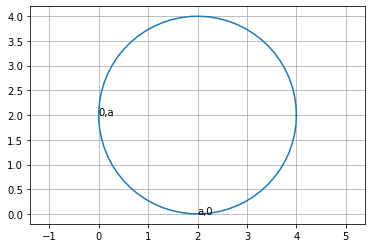
\includegraphics[width=\columnwidth]{./solutions/4/2/5/circle new.png}
\caption{Circle touching the co-ordinate axes \\a=2}
\label{eq:solutions/4/2/5/}
\end{figure}
